\documentclass{beamer}
\usepackage[lithuanian]{babel}
\usepackage[utf8x]{inputenc}
\usepackage[L7x]{fontenc}
\usepackage{lmodern}
\usepackage{caption}
\usepackage{subfig}
\usepackage{graphicx}

\let\oldshorttitle\insertshorttitle
\renewcommand*\insertshorttitle{
    \leftskip=0.4cm
\oldshorttitle\hfill \insertframenumber\,/\,\inserttotalframenumber
}

\usetheme{Dresden}

\title[IBM MIRA]{IBM MIRA}
\author[M. Norkin]{Maksim Norkin, AKSfm-15}
\institute[VGTU Elektronikos fakultetas]{
  Vilniaus Gedimino technikos universitetas\\
  Elektronikos fakultetas\\
  Elektroninių sistemų katedra\\
  \texttt{maksim.norkin@stud.vgtu.lt}
}

\begin{document}

    \begin{frame}
        \titlepage
    \end{frame}

    \begin{frame}
        \begin{figure}[H]
            \centering
            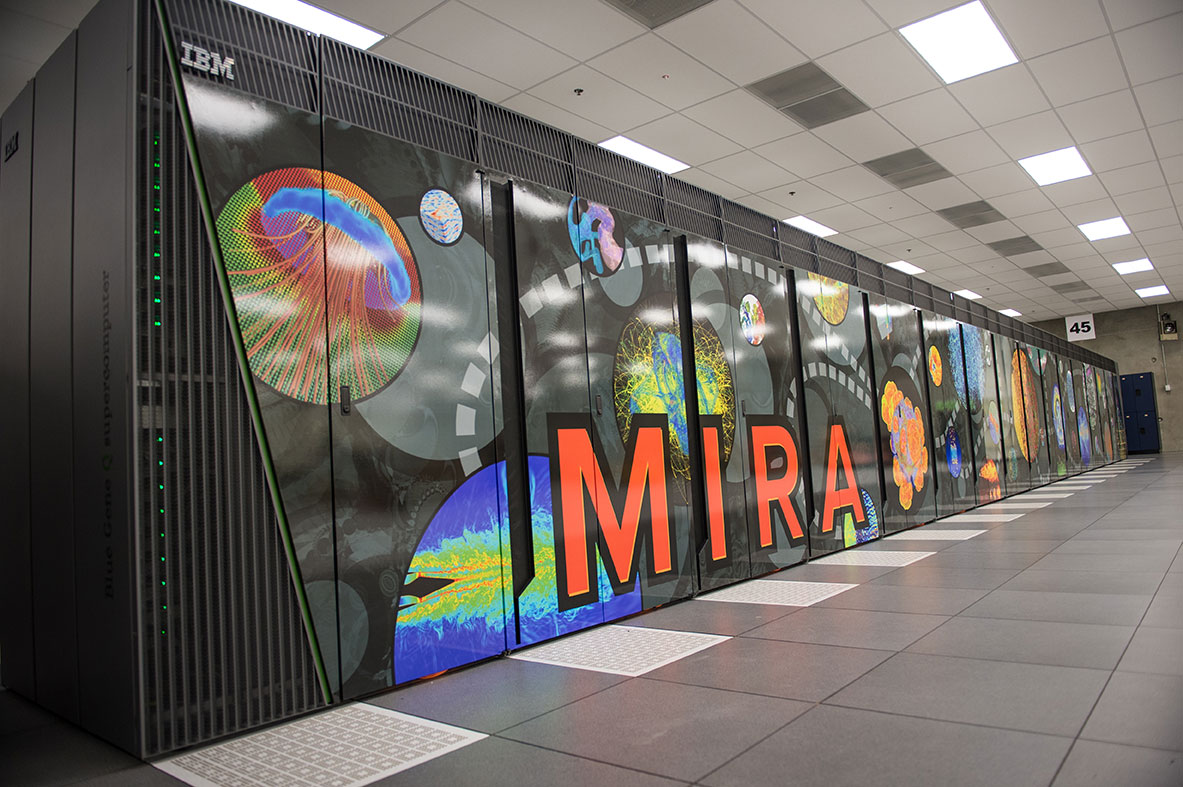
\includegraphics[width=280px]{img/mira.jpg}
            \caption{MIRA super kompiuteris}
        \end{figure}
    \end{frame}

    \begin{frame}
        Sudedamosios dalys
        \begin{itemize}
            \item Skaičiavimo mazgai
            \item Į/I mazgai
            \item Pagrindinis aptarnavimo mazgas
            \item Išorinio priėjimo mazgas
            \item Komunikacijos posistemė
        \end{itemize}
    \end{frame}

    \begin{frame}
        \begin{figure}[H]
            \centering
            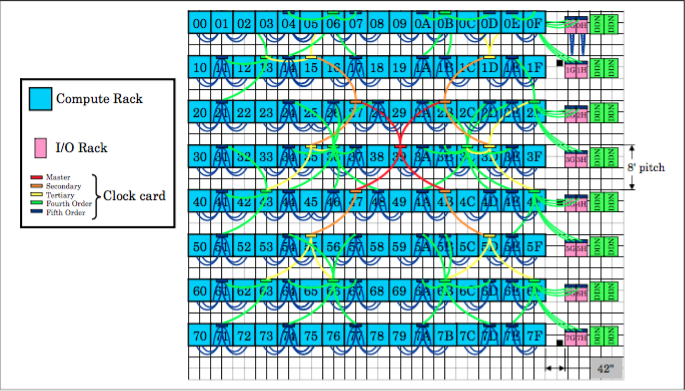
\includegraphics[width=280px]{img/cluster.png}
            \caption{Aukšto plano pavyzdys \cite{milano2013ibm}}
        \end{figure}
    \end{frame}

    \begin{frame}
        Skaičiavimo mazgo sandara:
        \begin{itemize}
            \item Korta
            \begin{itemize}
                \item 16 IBM Blue Gene/Q PowerPC A2 branduoliai
                \item 16 GB darbinės atminties
            \end{itemize}
            \item 32 kortos sudaro mazgo plokštę
            \item 16 mazgo plokščių sudaro vidurinę plokštę
        \end{itemize}
    \end{frame}

    \begin{frame}
        \begin{figure}[H]
            \centering
            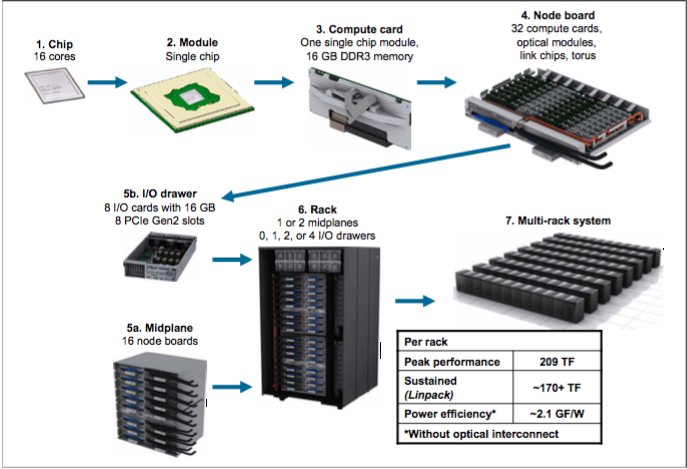
\includegraphics[width=280px]{img/rack-components.png}
            \caption{Apatarinės įrangos dalys \cite{milano2013ibm}}
        \end{figure}
    \end{frame}

    \begin{frame}
        \begin{figure}[H]
            \centering
            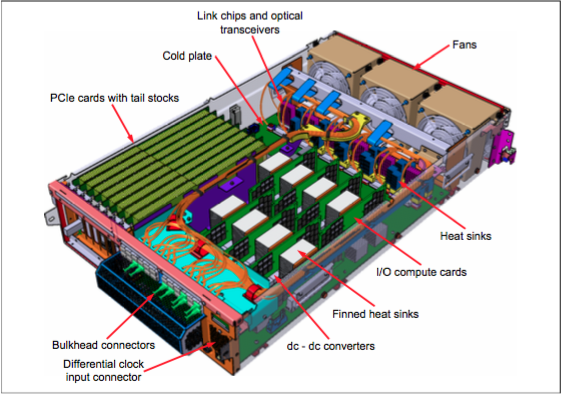
\includegraphics[width=280px]{img/internals.png}
            \caption{Į/I stalčiaus vaizdas \cite{milano2013ibm}}
        \end{figure}
    \end{frame}

    \begin{frame}
        \begin{itemize}
            \item 48 spintos
            \item 786 432 CPĮ
            \item 768 TB atminties
            \item 8.59 petaFLOPS (teorinis 10.06 petaFLOPS)
        \end{itemize}
    \end{frame}

    \begin{frame}
        \frametitle{Operacinė sistema}
        \begin{itemize}
            \item Naudojamas specializuotas Linux branduolys
            \item Pateikiamos bibliotekos darbui su gijomis, skaičiavimais, žinučių perdavimui
            \item Įrankiai programų skrodimui
        \end{itemize}
    \end{frame}

    \begin{frame}
        \begin{itemize}
            \item Taupus energijai
            \begin{itemize}
                \item Daug branduoliu vienam luste
                \item Vandens vėsinimo sistema
            \end{itemize}
            \item Per dieną galima atlikti tiek skaičiavimų, kiek eilinis kompiuteris atliks per 20 metų
            \item Pagrinde naudojamas mokslininkų, atlikti plataus mąsto simuliacijas
        \end{itemize}
    \end{frame}


    \begin{frame}
        \frametitle{Ačiū}

        Klausimai?

    \end{frame}

    \begin{frame}[allowframebreaks]
        \frametitle{Literatūra}
        
        \bibliographystyle{plain}
        \bibliography{references}
    \end{frame}

\end{document}